\documentclass{article}
\usepackage[utf8]{inputenc}
\usepackage[includeheadfoot, margin=1em,headheight=2em]{geometry}
\usepackage{titling}
\geometry{a4paper, left=2cm, right=2cm, top=2cm, bottom=2cm}
\usepackage{graphicx}
\usepackage{enumitem}
\providecommand{\versionnumber}{1.0.0}
\usepackage{array}
\usepackage[italian]{babel}
\newcolumntype{P}[1]{>{\centering\arraybackslash}p{#1}}
\renewcommand{\arraystretch}{1.5} % Default value: 1
\setlength{\droptitle}{-6em}
\usepackage{capt-of}

%font
\usepackage[defaultfam,tabular,lining]{montserrat}
\usepackage[T1]{fontenc}
\renewcommand*\oldstylenums[1]{{\fontfamily{Montserrat-TOsF}\selectfont #1}}

%custom bold 
\usepackage[outline]{contour}
\usepackage{xcolor}
\newcommand{\custombold}{\contour{black}}

%table colors
\usepackage{color, colortbl}
\definecolor{Blue}{rgb}{0.51,0.68,0.79}
\definecolor{LightBlue}{rgb}{0.82,0.87,0.90}
\definecolor{LighterBlue}{rgb}{0.93,0.95,0.96}

%Header
\usepackage{fancyhdr, xcolor}
\pagestyle{fancy}
\let\oldheadrule\headrule% Copy \headrule into \oldheadrule
\renewcommand{\headrule}{\color{Blue}\oldheadrule}% Add colour to \headrule
\renewcommand{\headrulewidth}{0.2em}
\fancyhead[L]{Analisi dei requisiti}
\fancyhead[C]{Cybersorceres}
\fancyhead[R]{versione \versionnumber}


\title{\Huge{\textbf{Analisi dei requisiti}}\vspace{-1em}}

\author{CyberSorcerers Team}
\date{}

 % Imposta labelformat=empty per nascondere il prefisso "Figura X:"
 \usepackage{caption}
\captionsetup[figure]{labelformat=empty}

\begin{document}
\maketitle

\vspace{-3em}
\begin{figure}[h]
  \centering
  
\includegraphics[width=6cm, height=6cm]{documenti/logo rotondo.png}
  \label{fig:immagine}
\end{figure}

\vspace{6em}
\large{

\begin{center}
    \begin{tabular}{l c c}
        \rowcolor{Blue} 
        \textbf{Informazioni sul documento} & &\\ [1 ex]
        \rowcolor{LighterBlue}
        Destinatari: & Prf. Tullio Vardanega & Prf. Riccardo Cardin\\ [1 ex]
    \end{tabular}
\end{center}}
\newpage
\custombold{Registro dei Cambiamenti - Changelog}

\begin{center}
\begin{tabular}{P{5em} P{5em} P{8em} P{8em} P{10em}} 
  \rowcolor{Blue}
    \custombold{Versione} & \custombold{Data} & \custombold{Autore} &
    \custombold{ Verificatore} & \custombold{Dettaglio}\\
    \rowcolor{LightBlue}
     0.1.1& 11/01/2024& Caniato Sabrina & Giulia Dentone & Aggiunta caption alle immagini\\ 
    \rowcolor{LighterBlue}
     0.1.0& 03/01/2024 & Caniato Sabrina &Vignotto Samuele & Sistemato l'analisi dei casi d'uso dopo il colloquio col Prof. R. Cardin. Aggiunta delle specifiche dei sottocasi d'uso.\\
    \rowcolor{LightBlue}
    0.0.1& 09/12/2023 & Caniato Sabrina  & Vignotto Samuele & Definizione struttura del documento e scheletro delle sezioni. Scrittura introduzione ed obiettivi delle diverse sezioni.\\ 
    \rowcolor{LighterBlue}
     0.0.1& 03/12/2023 & Vignotto Samuele & Lazzarin Nicola & Prima stesura dei casi d'uso e dell'analisi dei requisiti.\\
    
     
    
\end{tabular}
\end{center}
\newpage
\tableofcontents
\listoffigures
\newpage
\section*{Introduzione}

\subsection*{Scopo del documento}

Questo documento ha lo scopo di fornire una descrizione approfondita del prodotto, analizzando nel dettaglio i requisiti, ottenuti tramite incontri con l'azienda e analisi del capitolato. Quest'analisi si concretizza con l'individuazione di casi d'uso, punto centrale di questo documento.


\subsection*{Scopo del prodotto}
L'azienda proponente ha richiesto la creazione di una web app\textsubscript{G} che, tramite l'uso di IA\textsubscript{G} (in questo caso ChatGPT4 e Bedrock) è in grado di creare epic user stories\textsubscript{G} a partire dalle richieste del cliente e confrontarle con il codice sviluppato in modo da informare il cliente dello stato di avanzamento dello sviluppo del prodotto. Inoltre deve essere possibile, sia per il Project Manager\textsubscript{G}, sia per il cliente rilasciare dei feedback (nel primo caso riguardanti l'adeguatezza delle stories, nel secondo caso riguardanti il prodotto finale) al fine di migliorare l'IA\textsubscript{G}. È inoltre richiesta un' analisi comparativa tra le due IA utilizzate e lo sviluppo di un plugin\textsubscript{G} utile agli sviluppatori e al Project Manager\textsubscript{G}.

\subsection*{Glossario}
Alcuni termini presenti nel documento potrebbero essere ambigui, pertanto verranno inseriti nel Glossario v.1.0.0. La loro presenza all'interno di esso sarà indicata tramite una G maiuscola a pedice.

\section*{Casi d'uso}
\subsection*{Scopo}
Lo scopo di questa sezione è raccogliere tutti i casi d'uso\textsubscript{G} individuati, facendo riferimento alle funzionalità individuate durante la sessione di design thinking\textsubscript{G} fatta in collaborazione con l'azienda.

\subsection*{Attori}
Come si è evidenziato durante la sessione di design thinking\textsubscript{G} con i proponenti la web app\textsubscript{G} avrà necessità di tre diverse interfacce per essere usata adeguatamente da tutte le tipologie di attori\textsubscript{G}: clienti, sviluppatori e Project Manager\textsubscript{G}. L'IA\textsubscript{G}  (ChatGPT o Bedrock) viene considerata attore\textsubscript{G} secondario in quanto utilizzeremo un servizio che ci viene offerto. Inoltre è necessario lo sviluppo di un plugin\textsubscript{G} accessibile solamente a agli sviluppatori e al Project Manager\textsubscript{G}.\\\\

Per facilitare la comprensione del diagramma dei casi d'uso\textsubscript{G}  abbiamo utilizzato due generalizzazioni: Utente e Utente aziendale: 

\begin{figure}[h]
    \centering
    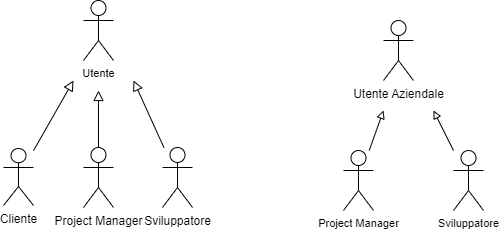
\includegraphics{./imgUML/Attori.png}
    \caption{Generalizzazione degli attori Utente ed Utente Aziendale}
    \label{fig:attori}
\end{figure}

\newpage
\custombold{UML Casi d'uso}
\begin{figure}[h]
    \centering
    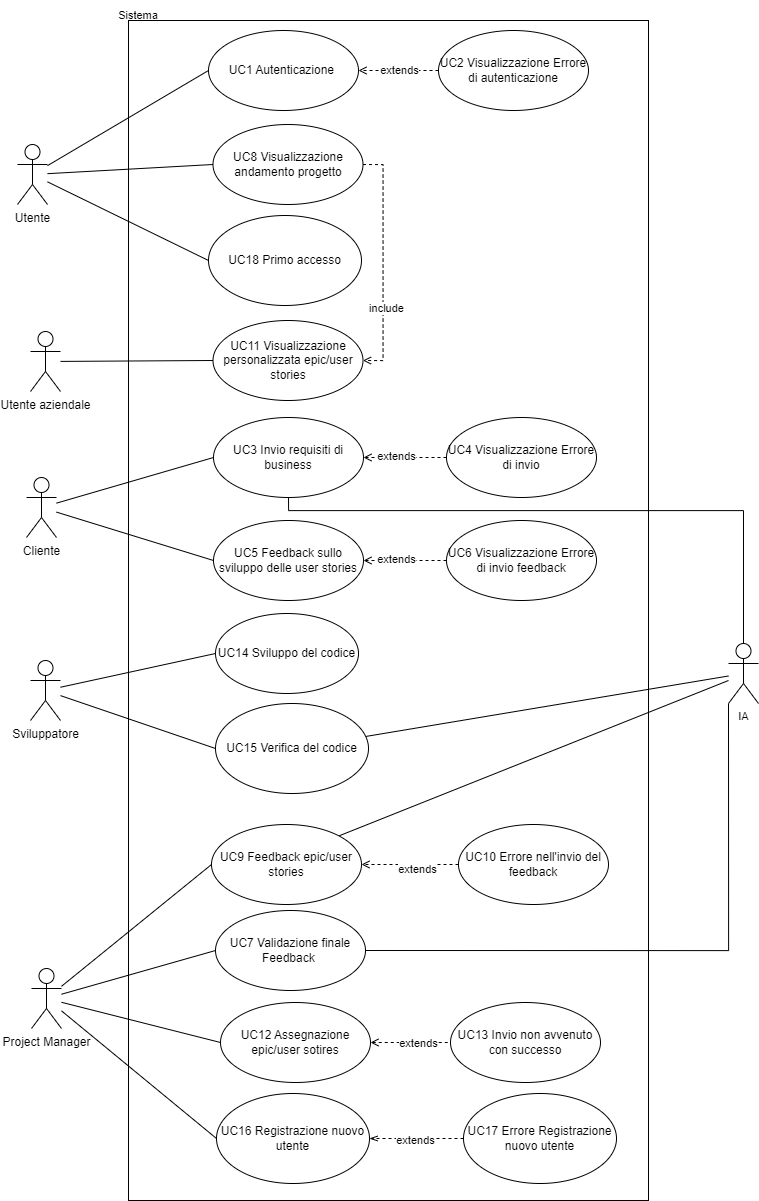
\includegraphics[height = 0.70\textheight]{./imgUML/UML.png}
    \caption{UML dei casi d'uso}
    \label{fig:UML}
\end{figure}
\newpage

\section{UC1-Autenticazione}
    \begin{figure}[h]
      \centering
      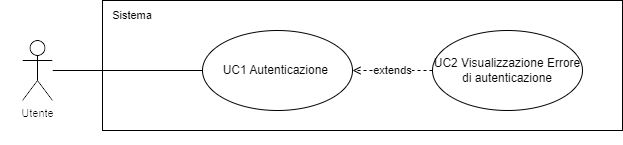
\includegraphics{./imgUML/UC1.png}
      \caption{UC1}
      \label{fig:UC1}
    \end{figure} 
    
     \subsection*{Main actor}
         \begin{itemize}
             \item Utente;
         \end{itemize}
     \subsection*{Preconditions} 
        \begin{itemize}
            \item Essere registrati nel sistema con i propri permessi
        \end{itemize}
               
    \subsection*{Postconitions}
        \begin{itemize}
            \item Utente riconosciuto dal sistema;
        \end{itemize}
    \subsection*{Main scenario}
        \begin{figure}[h]
            \centering
            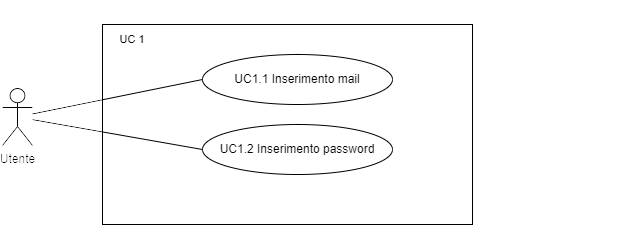
\includegraphics{./imgUML/UC1-zoom.png}
            \caption{Sottocasi UC1}
            \label{fig:UC1_sottocasi}
        \end{figure}
            
        \begin{itemize}
            \item Compilazione campo mail [UC1.1];
            \item Compilazione campo password [UC1.2];
        \end{itemize}
            
        \subsection*{Alternative scenario}
            \begin{itemize}
                \item Visualizzazione errore di autenticazione [UC2]
            \end{itemize}
            
\subsection{UC1.1-Inserimento Mail}
    
     \subsection*{Main actor}
         \begin{itemize}
             \item Utente;
         \end{itemize}
     \subsection*{Preconditions} 
        \begin{itemize}
            \item Essere registrati nel sistema con i propri permessi
            \item Trovarsi nella pagina di login
        \end{itemize}
        \subsection*{Postcondition} 
        \begin{itemize}
            \item Email inserita
        \end{itemize}

\subsection{UC1.2-Inserimento Password}
    
     \subsection*{Main actor}
         \begin{itemize}
             \item Utente;
         \end{itemize}
     \subsection*{Preconditions} 
        \begin{itemize}
            \item Essere registrati nel sistema con i propri permessi
            \item Trovarsi nella pagina di login
        \end{itemize}
        \subsection*{Postcondition} 
        \begin{itemize}
            \item Password inserita
            \item Possibilità di effettuare il login
        \end{itemize}

\section{UC2-Errore di autenticazione}
    
     \subsection*{Main actor}
         \begin{itemize}
             \item Utente;
         \end{itemize}
     \subsection*{Preconditions} 
        \begin{itemize}
            \item Essere registrati nel sistema con i propri permessi
        \end{itemize}
               
    \subsection*{Postconitions}
        \begin{itemize}
            \item Utente Non riconosciuto dal sistema;
        \end{itemize}
            
    
\section{UC3-Compilazione requisiti di business}
    \begin{figure}[h]
      \centering
      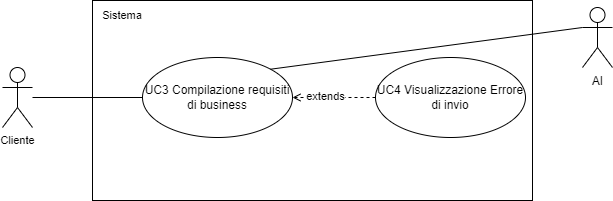
\includegraphics[width=.8\textwidth, height=.6\textheight, keepaspectratio]{./imgUML/UC3.png}
            \caption{UC3}
      \label{fig:UC3}
    \end{figure}
     \subsection*{Main actor}
     \begin{itemize}
         \item Cliente;
     \end{itemize}
      \subsection*{Second actor}
     \begin{itemize}
         \item Intelligenza Artificiale;
     \end{itemize}
     \subsection*{Preconditions} 
     \begin{itemize}
         \item Essere riconosciuti dal sistema come Cliente;
         \item Trovarsi nella sezione per aggiungere un nuovo requisito di business\textsubscript{G} 
     \end{itemize}
     \subsection*{Postconitions} 
        \begin{itemize}
            \item Invio dei requisiti di business all'intelligenza artificiale;
        \end{itemize}
        
     \subsection*{Main scenario}

        \begin{itemize}
            \item Stesura dei requisiti richiesti;
        \end{itemize}
     \subsection*{Alternative scenario}
        \begin{itemize}
            \item Messaggio d'errore durante l'invio [UC4]
        \end{itemize}

\section{UC4-Errore nell'invio dei requisiti di business}

     \subsection*{Main actor}
     \begin{itemize}
         \item Cliente;
     \end{itemize}
     \subsection*{Preconditions} 
     \begin{itemize}
         \item Essere riconosciuti dal sistema come Cliente;
         \item Trovarsi nella sezione per aggiungere un nuovo requisito di business\textsubscript{G} 
     \end{itemize}
     \subsection*{Postconditions} 
        \begin{itemize}
            \item Invio dei requisiti di business\textsubscript{G}  all'intelligenza artificiale non riuscito;
        \end{itemize}


\section{UC5-Feedback cliente sullo sviluppo user stories}
    \begin{figure}[h]
      \centering
      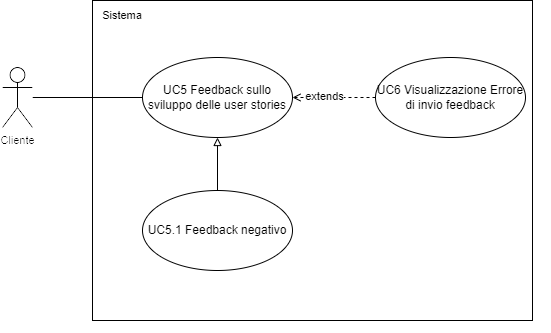
\includegraphics{./imgUML/UC5.png}
        \caption{UC5}
      \label{fig:UC5}
    \end{figure}
    
    \subsection*{Main actor}
    \begin{itemize}
        \item Cliente;
    \end{itemize}
    
    \subsection*{Preconditions}
    \begin{itemize}
        \item Essere riconosciuti dal sistema come Cliente;
        \item Presenza di almeno una user story\textsubscript{G}  o epic story\textsubscript{G} ;
        \item Epic stories completata;
        \item Trovarsi nella user story completata nella sezione apposita per l'invio del feedback;
    \end{itemize}
    
    \subsection*{Postconditions}
    \begin{itemize}
        \item Epic/user stories completato;
    \end{itemize}
    
    \subsection*{Main scenario}
        \begin{figure}[h]
            \centering
            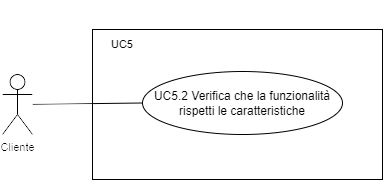
\includegraphics{./imgUML/UC5-zoom.png}
            \caption{Sottocasi UC5}
            \label{fig:UC5_sottocasi}
        \end{figure}
        \begin{itemize}
            \item Verifica che la funzionalità rispetti le caratteristiche [UC5.2];
        \end{itemize}
        
    \subsection*{Alternative scenario}
    \begin{itemize}
        \item Visualizzazione errore invio feedback[UC6];
    \end{itemize}

    \subsection*{Generalize}
    \begin{figure}[h]
            \centering
            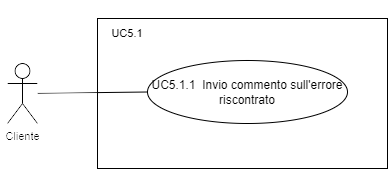
\includegraphics{./imgUML/UC5-zoom1.png}
            \caption{Generalizzazione del UC5}
            \label{fig:UC5_generalizzazione}
        \end{figure}
    \subsection{UC5.1 Feedback negativo}
    \begin{itemize}
            \item Invio commento sull'errore riscontrato [UC5.1.1];
        \end{itemize}
        
\section{UC6-Errore nell'invio del feedback}

     \subsection*{Main actor}
     \begin{itemize}
         \item Cliente;
     \end{itemize}
     \subsection*{Preconditions} 
 \begin{itemize}
        \item Essere riconosciuti dal sistema come Cliente;
        \item Presenza di almeno una user story\textsubscript{G}  o epic story\textsubscript{G} ;
        \item Epic stories\textsubscript{G}  completata;
        \item Trovarsi nella user story\textsubscript{G}  completata nella sezione apposita per l'invio del feedback;
    \end{itemize}
     \subsection*{Postconitions} 
        \begin{itemize}
            \item Invio del feedback al Project Manager\textsubscript{G}  non riuscito;
        \end{itemize} 

        
\section{UC7- Validazione finale del feedback}

\begin{figure}[h]
      \centering
      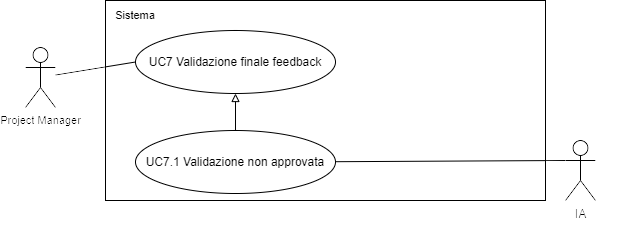
\includegraphics{./imgUML/UC7.png}
        \caption{UC7}
      \label{fig:UC7}
    \end{figure}
    
    \subsection*{Main actor}
    \begin{itemize}
        \item Project Manager\textsubscript{G} ;
    \end{itemize}
    
    \subsection*{Preconditions}
    \begin{itemize}
        \item Aver ricevuto dal Cliente un feedback negativo riguardante il lavoro finito;
        \item Presenza di almeno una user story\textsubscript{G}  o epic story\textsubscript{G} ;
        \item Epic stories\textsubscript{G}  completata;
    \end{itemize}
    
    \subsection*{Postconditions}
    \begin{itemize}
        \item Epic/user stories\textsubscript{G}  completato;
        \item Feedback per epic/user stories\textsubscript{G}  ricevuto dal sistema; 
    \end{itemize}
    
    \subsection*{Main scenario}
        \begin{figure}[h]
            \centering
            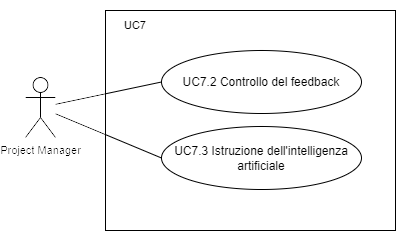
\includegraphics{./imgUML/UC7-zoom.png}
            \caption{Sottocasi UC7}
            \label{fig:UC7_sottocasi}
        \end{figure}
        \begin{itemize}
            \item Controllo del feedback inviato [UC7.2];
            \item Istruzione dell'intelligenza artificiale [UC7.3];
        \end{itemize}
        
    \subsection*{Generalize}
      \begin{figure}[h]
            \centering
            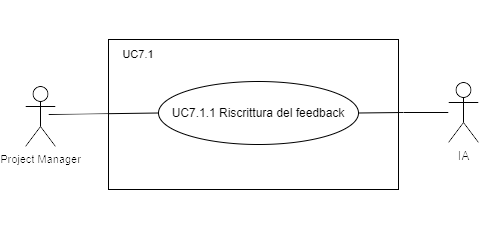
\includegraphics{./imgUML/UC7-zoom1.png}
            \caption{Generalizzazione del UC7}
            \label{fig:UC7_generalizzazione}
        \end{figure}
    \subsection{UC7.1 Validazione del feedback non approvata}
    \begin{itemize}
        \item Riscrittura del feedback da parte del Project Manager\textsubscript{G}  [UC7.1.1];
        \subsection*{UC7.1.1 Riscrittura del feedback da parte del Project Manager\textsubscript{G} }
     \subsection*{Main actor}
         \begin{itemize}
             \item Project Manager\textsubscript{G};
         \end{itemize}
     \subsection*{Preconditions} 
        \begin{itemize}
            \item Aver ricevuto un feedback negativo dal cliente;
            \item Il feedback non è comprensibile dall'intelligenza artificiale;
        \end{itemize}
        \subsection*{Postcondition} 
        \begin{itemize}
            \item Il feedback è scritto in modo comprensibile dall'intelligenza artificiale;
        \end{itemize}
    \end{itemize}
    
\subsection{UC7.2-Controllo del feedback inviato}
    
     \subsection*{Main actor}
         \begin{itemize}
             \item Cliente;
         \end{itemize}
     \subsection*{Preconditions} 
        \begin{itemize}
            \item Aver ricevuto un feedback negativo dal cliente;
        \end{itemize}
        \subsection*{Postcondition} 
        \begin{itemize}
            \item Il feedback è scritto in modo comprensibile dall'intelligenza artificiale;
        \end{itemize}
\subsection{UC7.3-Istruzione dell'intelligenza artificiale}
    
     \subsection*{Main actor}
         \begin{itemize}
             \item Cliente;
         \end{itemize}
     \subsection*{Preconditions} 
        \begin{itemize}
            \item Avere un feedback scritto in modo comprensibile dall'intelligenza artificiale;
        \end{itemize}
        \subsection*{Postcondition} 
        \begin{itemize}
            \item L'intelligenza artificiale è stata istruita grazie al feedback ricevuto;
        \end{itemize}

\section{UC8-Visualizzazione andamento progetto}
    \begin{figure}[h]
      \centering
      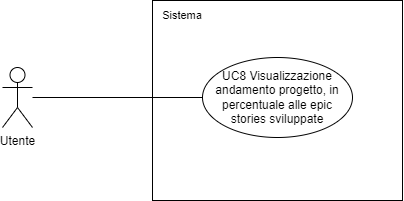
\includegraphics{./imgUML/UC8.png}
        \caption{UC8}
      \label{fig:UC8}
    \end{figure}
    
    \subsection*{Main actor}
        \begin{itemize}
            \item Utente; 
        \end{itemize}
        
    \subsection*{Preconditions}
        \begin{itemize}
            \item Essere riconosciuti dal sistema con i propri privilegi;
            \item Cliente ha inviato con successo i requisiti di business\textsubscript{G} al sistema;
            \item Requisiti di business\textsubscript{G} sono stati elaborati dal sistema;
            \item Project Manager\textsubscript{G} ha accettato le epic/user stories\textsubscript{G} generate dal sistema;
            \item Project Manager\textsubscript{G} ha assegnato le epic/user stories\textsubscript{G} agli Sviluppatori;
        \end{itemize}
        
    \subsection*{Postconitions}
        \begin{itemize}
            \item Presa visione dell'andamento del progetto;
        \end{itemize}
        
    \subsection*{Main scenario}
        
        \begin{itemize}
            \item Visualizzazione della percentuale rappresentante il quantitativo di epic/user stories\textsubscript{G} sviluppate;
        \end{itemize}
        

\section{UC9-Feedback epic/user stories\textsubscript{G} Project Manager\textsubscript{G}}
    \begin{figure}[h]
      \centering
      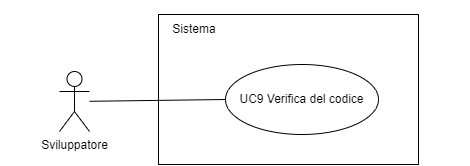
\includegraphics{./imgUML/UC9.png}
    \caption{UC9}      
      \label{fig:UC9}
    \end{figure}
%con feedback si intende un effetto di reazione prodotto da un messaggio su chi lo ha emesso
    \subsection*{Main actor}
    \begin{itemize}
        \item Project Manager\textsubscript{G};
    \end{itemize}
    \subsection{Second actor}
    \begin{itemize}
        \item Intelligenza artificiale;
    \end{itemize}
    
    \subsection*{Preconditions}
        \begin{itemize}
            \item Essere riconosciuti dal sistema come Project Manager\textsubscript{G};
            \item Cliente ha inviato con successo i requisiti di business\textsubscript{G} al sistema;
            \item Requisiti di business\textsubscript{G} sono stati elaborati dal sistema;
        \end{itemize}
        
    \subsection*{Postconditions}
        \begin{itemize}
            \item Feedback per epic/user stories ricevuto dal sistema;
            \item Il sistema ha generato epic/user stories\textsubscript{G} corrette, con corrispettivo tag\textsubscript{G};
        \end{itemize}
        
    \subsection*{Main scenario}
        \begin{figure}[h]
          \centering
          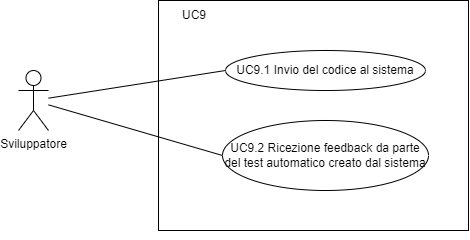
\includegraphics{./imgUML/UC9-zoom.png}
          \caption{Sottocasi UC9}
          \label{fig:UC9_sottocasi}
        \end{figure}

        \begin{itemize}
            \item Project Manager\textsubscript{G} visualizza epic/user stories\textsubscript{G} generate dal sistema [UC9.1];
            \item Project Manager\textsubscript{G} invia il feedback al sistema [UC9.2];
        \end{itemize}
        
    \subsection*{Alternative scenario}
        
        \begin{itemize}
            \item Errore nell'invio del feedback[UC10];
        \end{itemize}
        
\section{UC10-Errore nell'invio del feedback}

     \subsection*{Main actor}
     \begin{itemize}
         \item Project Manager\textsubscript{G};
     \end{itemize}
   \subsection*{Preconditions}
        \begin{itemize}
            \item Essere riconosciuti dal sistema come Project Manager\textsubscript{G};
            \item Cliente ha inviato con successo i requisiti di business\textsubscript{G} al sistema;
            \item Requisiti di business\textsubscript{G} sono stati elaborati dal sistema;
        \end{itemize}
        
    \subsection*{Postconitions}
        \begin{itemize}
            \item Feedback per epic/user stories\textsubscript{G} ricevuto dal sistema;
            \item Il sistema ha generato epic/user stories corrette\textsubscript{G}, con corrispettivo tag\textsubscript{G};
        \end{itemize} 

  
\section{UC11-Visualizzazione personalizzata epic/user stories\textsubscript{G}}
    \begin{figure}[h]
      \centering
      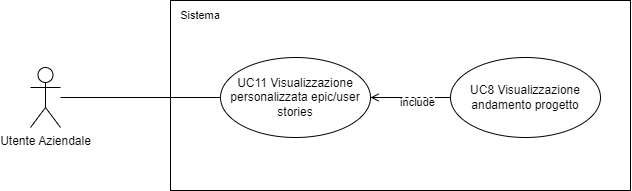
\includegraphics[width=.8\textwidth, height=.6\textheight, keepaspectratio]{./imgUML/UC11.png}
        \caption{UC11}
      \label{fig:UC11}
    \end{figure}
    
    \subsection*{Main actor}
        \begin{itemize}
            \item Utente Aziendale;
        \end{itemize}
        
    \subsection*{Preconditions}
        \begin{itemize}
            \item Essere riconosciuti dal sistema con i propri permessi;
            \item Cliente ha inviato con successo i requisiti di business\textsubscript{G} al sistema;
            \item requisiti di \textsubscript{G} sono stati elaborati dal sistema;
            \item Project Manager\textsubscript{G} ha accettato le epic/user stories\textsubscript{G} generate dal sistema;
            \item Project Manager\textsubscript{G} ha assegnato le epic/user stories\textsubscript{G} agli Sviluppatori;
        \end{itemize}
        
    \subsection*{Postconitions}
    \begin{itemize}
        \item Project Manager\textsubscript{G} ha preso visione dell'andamento del progetto;
    \end{itemize}
    
    \subsection*{Main scenario}
        \begin{itemize}
            \item Project Manager\textsubscript{G} visualizza la lista delle epis/user stories\textsubscript{G} assegnate;
        \end{itemize}
        
    \subsection*{Inclusione}
        \begin{itemize}
            \item Visualizzazione andamento progetto [UC8];
        \end{itemize}

\section{UC12-Assegnazione epic/user stories \textsubscript{G}}
    \begin{figure}[h]
      \centering
      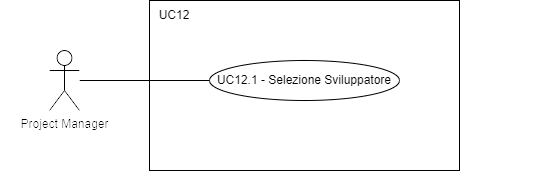
\includegraphics{./imgUML/UC12.png}
    \caption{UC12}
      \label{fig:UC12}
    \end{figure}

    \subsection*{Main actor}
    \begin{itemize}
        \item Project Manager\textsubscript{G};
    \end{itemize}
    
    \subsection*{Preconditions}
        \begin{itemize}
            \item Essere riconosciuto dal sistema come Project Manager\textsubscript{G};
            \item Le epic/user stories\textsubscript{G} che si vogliono assegnare devono avere feedback positivo;
            \item Trovarsi nella pagina della epic story\textsubscript{G} da assegnare;
        \end{itemize}
        
    \subsection*{Postconditions}
        \begin{itemize}
            \item Una o più epic/user stories\textsubscript{G} con feedback positivo è stata assegnata ad uno o più Sviluppatori;
        \end{itemize}
    
    \subsection*{Main scenario}
        \begin{figure}[h]
          \centering
          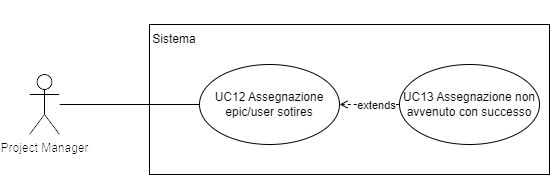
\includegraphics{./imgUML/UC12-zoom.png}
          \caption{Sottocasi UC12}
          \label{fig:UC12_sottocasi}
        \end{figure}
        
        \begin{itemize}
            \item Project Manager\textsubscript{G} seleziona lo Sviluppatore a cui assegnare la epic/user stories\textsubscript{G} selezionata [UC12.1];
        \end{itemize}
        
    \subsection*{Alternative scenario}
        \begin{itemize}
            \item Errore nell'assegnazione dell'epic story\textsubscript{G} [UC13]
        \end{itemize}    
        
    \subsection{UC12.1- Selezione dello sviluppatore}
        \subsection*{Main actor}
    \begin{itemize}
        \item Project Manager\textsubscript{G};
    \end{itemize}
    
    \subsection*{Preconditions}
        \begin{itemize}
            \item Essere riconosciuto dal sistema come Project Manager\textsubscript{G};
            \item Le epic/user stories\textsubscript{G} che si vogliono assegnare devono avere feedback positivo;
            \item Trovarsi nella pagina della epic story\textsubscript{G} da assegnare;
        \end{itemize}
        
    \subsection*{Postconditions}
        \begin{itemize}
            \item Una o più epic/user stories\textsubscript{G} con feedback positivo è stata assegnata ad uno o più Sviluppatori;
        \end{itemize}

\section{UC13- Assegnazione non avvenuta}

       \subsection*{Main actor}
    \begin{itemize}
        \item Project Manager\textsubscript{G};
    \end{itemize}
    
    \subsection*{Preconditions}
        \begin{itemize}
            \item Essere riconosciuto dal sistema come Project Manager\textsubscript{G};
            \item Le epic/user stories\textsubscript{G} che si vogliono assegnare devono avere feedback positivo;
            \item Trovarsi nella pagina della epic story\textsubscript{G} da assegnare;
        \end{itemize}
        
    \subsection*{Postconditions}
        \begin{itemize}
            \item L'assegnazione non è avvenuta con successo;
        \end{itemize}
    
\section{UC14-Sviluppo del codice}
    \begin{figure}[h]
      \centering
      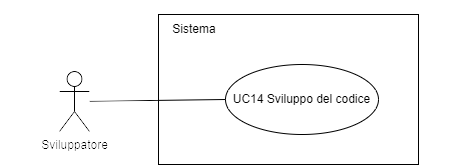
\includegraphics{./imgUML/UC14.png}
    \caption{UC14}
      \label{fig:UC14}
    \end{figure}
    
    \subsection*{Main actor}
        \begin{itemize}
            \item Sviluppatore;
        \end{itemize}
    
    \subsection*{Preconditions}
        \begin{itemize}
            \item Essere riconosciuti dal sistema come Sviluppatore;
            \item Avere un'assegnazione per quella user story\textsubscript{G} dal Project Manager\textsubscript{G};
        \end{itemize}
        
    \subsection*{Postconditions} 
        \begin{itemize}
            \item Il codice sviluppato e pronto per il testing\textsubscript{G};
            \item Il codice è correttamente taggato\textsubscript{G};  
        \end{itemize}
    
    \subsection*{Main scenario}
        \begin{figure}[h]
          \centering
          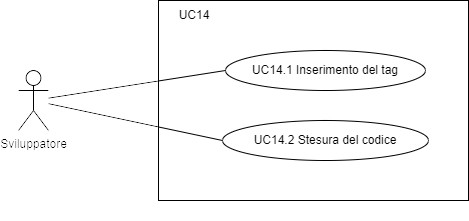
\includegraphics{./imgUML/UC14-zoom.png}
          \caption{Sottocasi UC14}
          \label{fig:UC14_sottocasi}
        \end{figure}
        
        \begin{itemize}
            \item Sviluppatore inserisce il tag\textsubscript{G} di riferimento alla user story\textsubscript{G} [UC14.1];
            \item Sviluppatore scrive del codice [UC14.2];
        \end{itemize}

        \subsection{UC14.1 Inserimento del Tag\textsubscript{G}}
\subsection*{Main actor}
        \begin{itemize}
            \item Sviluppatore;
        \end{itemize}
    
    \subsection*{Preconditions}
        \begin{itemize}
            \item Essere riconosciuti dal sistema come Sviluppatore;
            \item Avere un'assegnazione per quella user story dal Project Manager\textsubscript{G};
        \end{itemize}
        
    \subsection*{Postconditions} 
        \begin{itemize}
            \item Il codice è correttamente taggato\textsubscript{G};  
        \end{itemize}

        
        \subsection{UC14.2 Stesura del codice}
\subsection*{Main actor}
        \begin{itemize}
            \item Sviluppatore;
        \end{itemize}
    
    \subsection*{Preconditions}
        \begin{itemize}
            \item Essere riconosciuti dal sistema come Sviluppatore;
            \item Avere un'assegnazione per quella user story dal Project Manager\textsubscript{G};
        \end{itemize}
        
    \subsection*{Postconditions} 
        \begin{itemize}
            \item Il codice sviluppato e pronto per il testing\textsubscript{G};
        \end{itemize}
        
\section{UC15-Verifica codice da parte dell'IA\textsubscript{G}}
    \begin{figure}[h]
      \centering
      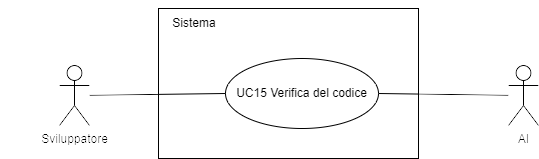
\includegraphics{./imgUML/UC15.png}
        \caption{UC15}
      \label{fig:UC15}
    \end{figure}
    
    \subsection*{Main actor}
        \begin{itemize}
            \item Sviluppatore;
        \end{itemize}
    \subsection*{Second actor}
        \begin{itemize}
            \item Intelligenza Artificiale;
        \end{itemize}
    
    \subsection*{Preconditions}
        \begin{itemize}
            \item Essere riconosciuti dal sistema come Sviluppatore;
            \item Cliente ha inviato requisiti di business\textsubscript{G};
            \item Project Manager\textsubscript{G} ha accettato epic/user stories\textsubscript{G};
            \item Project Manager\textsubscript{G} ha assegnato epic/user stories\textsubscript{G};
            \item Sviluppatore ha sviluppato codice e test\textsubscript{G} riguardante una o più user story\textsubscript{G};
            \item Sviluppatore ha taggato\textsubscript{G} correttamente il codice;
        \end{itemize}
        
    \subsection*{Postconditions}
        \begin{itemize}
            \item Sviluppatore riceve feedback da parte del sistema riguardante il codice inviato;
        \end{itemize}
    
    \subsection*{Main scenario}
        \begin{figure}[h]
          \centering
          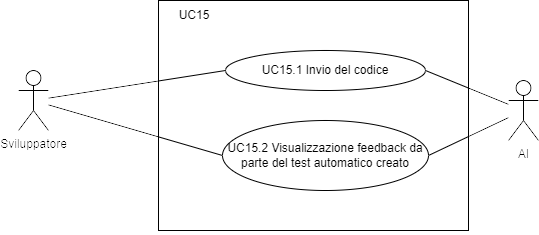
\includegraphics{./imgUML/UC15-zoom.png}
          \caption{Sottocasi UC15}
          \label{fig:UC15_sottocasi}
        \end{figure}
        
        \begin{itemize}
            \item Sviluppatore invia codice per la verifica [UC15.1];

            \item Sviluppatore riceve feedback dal sistema riguardante il codice inviato [UC15.2];
        \end{itemize}
        
    \subsection{UC15.1- Invio codice per la verifica}
    \subsection*{Main actor}
        \begin{itemize}
            \item Sviluppatore;
        \end{itemize}
        
    \subsection*{Preconditions}
        \begin{itemize}
            \item Essere riconosciuti dal sistema come Sviluppatore;
            \item Cliente ha inviato requisiti di business\textsubscript{G};
            \item Project Manager\textsubscript{G} ha accettato epic/user stories\textsubscript{G};
            \item Project Manager\textsubscript{G} ha assegnato epic/user stories\textsubscript{G};
            \item Sviluppatore ha sviluppato codice e test\textsubscript{G} riguardante una o più user story\textsubscript{G};
            \item Sviluppatore ha taggato\textsubscript{G} correttamente il codice;
        \end{itemize}
        
    \subsection{UC15.2- Visualizzazione feedback}
    \subsection*{Main actor}
        \begin{itemize}
            \item Sviluppatore;
        \end{itemize}
        
    \subsection*{Preconditions}
        \begin{itemize}
            \item Essere riconosciuti dal sistema come Sviluppatore;
            \item Cliente ha inviato requisiti di business\textsubscript{G};
            \item Project Manager\textsubscript{G} ha accettato epic/user stories\textsubscript{G};
            \item Project Manager\textsubscript{G} ha assegnato epic/user stories\textsubscript{G};
            \item Sviluppatore ha sviluppato codice e test\textsubscript{G} riguardante una o più user story\textsubscript{G};
            \item Sviluppatore ha taggato\textsubscript{G} correttamente il codice;
        \end{itemize}
        
    \subsection*{Postconditions}
        \begin{itemize}
            \item Sviluppatore riceve feedback da parte del sistema riguardante il codice inviato;
            \item Il codice può essere sistemato, in base a quello consigliato dall'intelligenza artificiale;
        \end{itemize}
    

        
\section{UC16-Inserimento di un nuovo cliente}
    \begin{figure}[h]
      \centering
      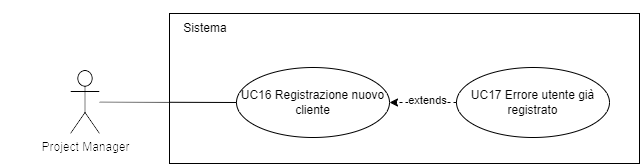
\includegraphics{./imgUML/UC16.png}
    \caption{UC16}
      \label{fig:UC16}
    \end{figure}
    
    \subsection*{Main actor}
        \begin{itemize}
            \item Project Manager\textsubscript{G};
        \end{itemize}
        
    \subsection*{Preconditions}
        \begin{itemize}
            \item Essere riconosciuti dal sistema come Project Manager\textsubscript{G};
            \item Cliente ha preso contatto con l'azienda per l'inizio di un nuovo progetto insieme;
        \end{itemize}
        
    \subsection*{Postconditions}
        \begin{itemize}
            \item Cliente registrato nel sistema;
            \item Cliente può effettuare il primo accesso;
        \end{itemize}
    
    \subsection*{Main scenario}
        \begin{figure}[h]
          \centering
          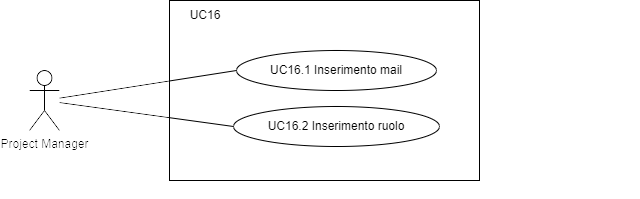
\includegraphics{./imgUML/UC16-zoom.png}
          \caption{Sottocasi UC16}
          \label{fig:UC16_sottocasi}
        \end{figure}
        
        \begin{itemize}
            \item Il Project Manager\textsubscript{G} inserisce mail [UC16.1];
            \item Il Project Manager\textsubscript{G} inserisce ruolo di Cliente [UC16.2];
        \end{itemize}
        
    \subsection*{Alternative scenario}
        \begin{itemize}
            \item Errore nella registrazione dell'utente [UC17];
        \end{itemize}

    \subsection{UC16.1- Inserimento Mail}
    \subsection*{Main actor}
        \begin{itemize}
            \item Project Manager\textsubscript{G};
        \end{itemize}
        
    \subsection*{Preconditions}
        \begin{itemize}
            \item Essere riconosciuti dal sistema come Project Manager\textsubscript{G};
            \item Cliente ha preso contatto con l'azienda per l'inizio di un nuovo progetto insieme;
        \end{itemize}
        

    \subsection{UC16.2- Inserimento ruolo}
    \subsection*{Main actor}
        \begin{itemize}
            \item Project Manager\textsubscript{G};
        \end{itemize}
        
    \subsection*{Preconditions}
        \begin{itemize}
            \item Essere riconosciuti dal sistema come Project Manager\textsubscript{G};
            \item Cliente ha preso contatto con l'azienda per l'inizio di un nuovo progetto insieme;
        \end{itemize}
        
    \subsection*{Postconditions}
        \begin{itemize}
            \item Cliente registrato nel sistema;
            \item Cliente può effettuare il primo accesso;
        \end{itemize}

\section{UC17- Errore nella registrazione dell'utente}
\subsection*{Main actor}
        \begin{itemize}
            \item Project Manager\textsubscript{G};
        \end{itemize}
        
    \subsection*{Preconditions}
        \begin{itemize}
            \item Essere riconosciuti dal sistema come Project Manager\textsubscript{G};
            \item Cliente ha preso contatto con l'azienda per l'inizio di un nuovo progetto insieme;
        \end{itemize}
        
    \subsection*{Postconditions}
        \begin{itemize}
            \item Cliente non è registrato nel sistema;
        \end{itemize}
\section{UC18- Primo accesso}
 \begin{figure}[h]
          \centering
          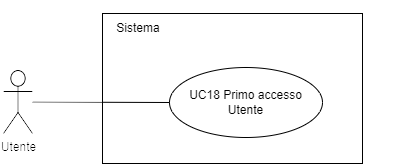
\includegraphics{./imgUML/UC18.png}
            \caption{UC18}
          \label{fig:UC18}
        \end{figure}
\subsection*{Main actor}
        \begin{itemize}
            \item Utente;
        \end{itemize}
        
    \subsection*{Preconditions}
        \begin{itemize}
            \item Essere riconosciuti dal sistema con il proprio ruolo;
            \item Non aver ancora effettuato il primo accesso;
        \end{itemize}
        
    \subsection*{Postconditions}
        \begin{itemize}
            \item Cliente registrato nel sistema con la nuova password;
            \item Cliente può iniziare a scrivere i suoi requisisti di business\textsubscript{G};
        \end{itemize}
     \subsection*{Main scenario}
        \begin{figure}[h]
          \centering
          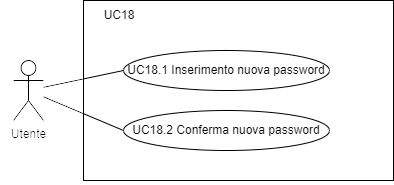
\includegraphics{./imgUML/UC18-zoom.png}
            \caption{Sottocasi UC18}
          \label{fig:UC18_sottocasi}
        \end{figure}
        
        \begin{itemize}
            \item Inserimento nuova password [UC18.1];
            \item Conferma nuova password [UC18.2];
        \end{itemize}

        \subsection{UC18.1 Inserimento nuova password}
            \subsection*{Main actor}
        \begin{itemize}
            \item Utente;
        \end{itemize}
        
    \subsection*{Preconditions}
        \begin{itemize}
            \item Essere riconosciuti dal sistema con il proprio ruolo;
            \item Non aver ancora effettuato il primo accesso;
        \end{itemize}

    \subsection{UC18.2- Conferma nuova password}
    \subsection*{Main actor}
        \begin{itemize}
            \item Utente;
        \end{itemize}
        
    \subsection*{Preconditions}
        \begin{itemize}
            \item Essere riconosciuti dal sistema con il proprio ruolo;
            \item Non aver ancora effettuato il primo accesso;
        \end{itemize}
        
    \subsection*{Postconditions}
        \begin{itemize}
            \item Cliente registrato nel sistema con la nuova password;
            \item Cliente può iniziare a scrivere i suoi requisisti di business\textsubscript{G};
        \end{itemize}

\newpage
\section{Requisiti}
\subsection{Requisiti funzionali}
\begin{center}
    \begin{tabular}{|p{3cm}|p{6cm}|p{3,5cm}|p{3cm}|}
    \rowcolor{Blue} 
\hline
Classificazione & Descrizione & Indirizzato a&Codice  \\ 
\rowcolor{LightBlue}
\hline
Obbligatorio & Accesso a web app\textsubscript{G} tramite login composto da email e password & Sviluppatore, Cliente, Project Manager\textsubscript{G} & UC1, UC16, UC18 \\ 
\rowcolor{LighterBlue}
\hline
Obbligatorio & Scrittura di richieste di buisness\textsubscript{G} tramite box testuale da web app\textsubscript{G} & Cliente & UC3\\ 
\rowcolor{LightBlue}
\hline
Obbligatorio & Invio delle richieste di buisness\textsubscript{G} da web app\textsubscript{G} & Cliente & UC3\\
\hline
\rowcolor{LighterBlue}

Obbligatorio & Visualizzazione andamento sviluppo richieste tramite barra di completamento basata sulla percentuale di user stories\textsubscript{G} completate & Cliente, Project Manager\textsubscript{G} & UC8, UC11\\
\rowcolor{LightBlue}
\hline
Obbligatorio & Approvazione o rifiuto del risultato relativo all'implementazione di una user story\textsubscript{G} & Cliente & UC5\\
\hline
\rowcolor{LighterBlue}

Desiderabile & Ricezione notifiche quando user story\textsubscript{G} completata & Cliente & UC5 UC8\\
\hline
\rowcolor{LightBlue}
\hline
Obbligatorio & Funzionalità di tag\textsubscript{G} nel plugin\textsubscript{G}  & Sviluppatore & UC14\\
\hline
\rowcolor{LighterBlue}

Obbligatorio & Lista di user stories\textsubscript{G} assegnate da Project Manager\textsubscript{G} sia su web app\textsubscript{G} che su plugin\textsubscript{G} & Sviluppatore & UC14 UC15\\
\hline
\rowcolor{LightBlue}

Desiderabile & Ricezione notifica su web app\textsubscript{G} quando nuova user story\textsubscript{G} è assegnata dal Project Manager\textsubscript{G}& Sviluppatore & UC12\\
\hline
\rowcolor{LighterBlue}
Obbligatorio & Invio del codice sviluppato a IA\textsubscript{G} per richiesta verifica& Sviluppatore & UC15\\

\hline
\rowcolor{LightBlue}

Obbligatorio & Visualizzazione users stories\textsubscript{G} generate da IA\textsubscript{G}  & Project Manager\textsubscript{G} & UC9\\
\hline


\end{tabular}

    \begin{tabular}{|p{3cm}|p{6cm}|p{3,5cm}|p{3cm}|}
    \rowcolor{Blue} 
\hline
Classificazione & Descrizione & Indirizzato a&Casi d'uso  \\ 
\rowcolor{LightBlue}
\hline
Obbligatorio & Invio di feedback sulle user stories\textsubscript{G} generate all'IA\textsubscript{G}& Project Manager\textsubscript{G}&UC9\\
\hline
\rowcolor{LighterBlue}

Obbligatorio & Suddivisione delle user stories\textsubscript{G} troppo grandi  & Project Manager\textsubscript{G}& UC9\\
\hline
\rowcolor{LightBlue}

Obbligatorio & Assegnazione user stories\textsubscript{G} agli sviluppatori& Project Manager\textsubscript{G}& UC12\\
\hline
\rowcolor{LighterBlue}

Desiderabile & Ricezione notifiche quando user story\textsubscript{G} viene generata in seguito a richiesta del cliente & Project Manager\textsubscript{G} & UC7\\
\hline
\rowcolor{LightBlue}

Obbligatorio & Invio richiesta di modifiche realtive a user stories\textsubscript{G} a IA\textsubscript{G} prima di approvazione& Project Manager\textsubscript{G}& UC7\\
\hline
\rowcolor{LighterBlue}

Obbligatorio & Visualizzazione andamento epic/user stories\textsubscript{G} assegnate& Sviluppatore& UC11\\

\hline

\end{tabular}
\captionof{table}{Tabella dei requisiti funzionali}
\label{tab:reqfunz}
\end{center}

\subsection{Requisiti di qualità}
I requisiti di qualità, e attinenti alle richieste del committente e da lui revisionati,  descrivono le caratteristiche principali e come il sistema deve esibirsi, per soddisfare le esigenze dell'utente.

\begin{center}
    \begin{tabular}{|p{3cm}|p{6cm}|p{3,5cm}|p{3cm}|}
    \rowcolor{Blue} 
\hline
Codice & Descrizione & Fonti  \\ 
\rowcolor{LightBlue}
\hline
& &  \\ 
\rowcolor{LighterBlue}
\hline
 & & \\ 
\rowcolor{LightBlue}
\hline
 & & \\
\hline
\rowcolor{LighterBlue}

& & \\
\rowcolor{LightBlue}
\hline
& & \\
\hline
\rowcolor{LighterBlue}

 & & \\
\hline
\end{tabular}
\captionof{table}{Tabella dei requisiti di quailità}
\label{tab:reqal}
\end{center}



\subsection{Requisiti di vincolo}
Di seguito la specifica per i requisiti di vincolo, i quali descrivono i limiti e le restrizioni che un sistema
deve rispettare per soddisfare le esigenze dell'utente. 
\begin{center}

    \begin{tabular}{|p{3cm}|p{6cm}|p{3,5cm}|p{3cm}|}
    \rowcolor{Blue} 
\hline
Codice & Descrizione & Fonti  \\ 
\rowcolor{LightBlue}
\hline
& &  \\ 
\rowcolor{LighterBlue}
\hline
 & & \\ 
\rowcolor{LightBlue}
\hline
 & & \\
\hline
\rowcolor{LighterBlue}

& & \\
\rowcolor{LightBlue}
\hline
& & \\
\hline
\rowcolor{LighterBlue}

 & & \\
\hline

\end{tabular}
\captionof{table}{Tabella dei requisiti di vincolo}
\label{tab:reqvincolo}
\end{center}

\subsection{Requisiti sistemi operativi}


\subsection{Requisiti prestazionali}
Per un'applicazione eseguita su una web app\textsubscript{G}, i requisiti prestazionali possono essere influenzati dalle prestazioni del dispositivo dell'utente e la larghezza di banda della connessione Internet, Non vi sono particolari requisiti in questo senso, in quanto le tecnologie AWS e Chat GPT rispondono in modo ottimale a diverse esigenze:
\begin{itemize}
\item tempo ottimale di risposta;
\item scalabilità, evitando rallentamenti o anomalie non avendo problemi di gestione del carico 
\item utilizzo efficace delle risorse del sistema, riducendo larghezza di banda e non impegnando la memoria del dispositivo, 
\item disponibilità ed affidabilità
\end{itemize}

\subsection{Requisiti di sicurezza}







   
\end{document}